\section{Discusión}
En primer lugar, utilizamos el experimento 1 para poder analizar las variacion de la temperatura para cada angulo del horno. Graficamos los resultados obtenidos para cada radio para observar como se comporta la discipacion del calor en función del radio. De este modo, podriamos entender mejor como se comporta la función para sacar conclusiones de como obtener una mejor aproximacion para encontrar la isoterma pedida.

\begin{figure}[h]
  \center
  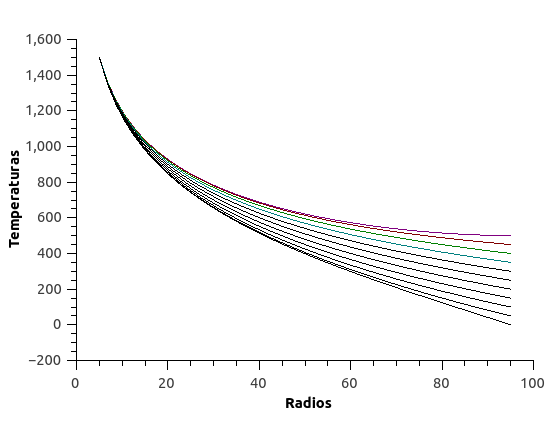
\includegraphics[scale=0.8]{imagenes/avanceTemperaturas.png}
  %\caption{La figura}
  \label{fig:avanceTemps}
\end{figure}

Cada curva corresponde a un angulo del horno y se grafica la temperatura para cada radio. Como se puede ver, se corresponden con la familia de funciones $f(x)= \frac{1}{x}$. De este modo, concluimos que utiliazar una regla de tres simple para aproximar la locación de la isoterma no es una aproximación correcta porque guarda una relación lineal, mientras que los datos revelan una relacion inversa multiplicativa. \\
Sin embargo, no resulta una tarea sencilla encontrar una mejor aproxiamción debido a que si la encontraramos, podriamos resolver el problema inicial sin tener que plantear el sistema de ecuaciones planteado anterior. Por tal razón, analizamos alternativas para encontrar una mejor aproximación. Para eso realizamos el experimento 3, para analizar como aumentando el nivel de discretización para una instancia dada, como impacta en el hallazgo de la isoterma. \\
Nuestra hipótesis era que aumentando el nivel de discretización, se refinara la locación de la isoterma, debido a la forma en que la hallamos es encontrar los dos puntos entre los que se encuentra la isoterma. Aumentando la cantidad de puntos, se disminuye la distancia entre los mismos, por lo que el error introducido por la aproximación también debe disminuir. \\
Nos encontramos con un resultado llamativo, que fue darnos cuenta que los primeros puntos no se correspondian con la funcion graficada, y algunos de los primeros puntos tenian un radio menor al radio al que tiende al función. Esto no debería suceder debido a lo siguiente: 
\newpage

\begin{wrapfigure}{l}{0.5\textwidth}
  \vspace{-20pt}
  \begin{center}
    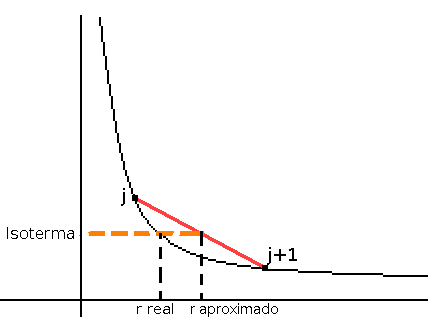
\includegraphics[scale=0.4]{imagenes/aprox.png}
  \end{center}
  \vspace{-20pt}
  \caption{Aproximación lineal contra valor esperado}
  \vspace{-10pt}
  \label{fig:aproximacion}
\end{wrapfigure}

Al utilizar una regla de tres simple, para cada radio obtenido deberíamos obtener un radio ligeramente mayor al radio real de la isoterma, debido a que la función de la discipación del calor tiene una relación inversa multiplicativa.\\
La razón por la que para los primeros valores la función se asemeja a una función lineal, es porque para los primeros casos la isoterma se encuentra entre el radio interno y el siguiente al radio interno. Basamos nuestra aproximación en contar con que el valor de la temperatura hasta el radio $j$ coincide con la función de discipación de calor, y a eso le introducimos un error al aproximar el radio que falta hasta la isoterma. Por lo tanto, si no contamos con valores anteriores al $j$, se cuenta con un error mayor, y la función se asimila más a una lineal que a la que queremos aproximar realmente.\\
Como se ve en la figura \ref{fig:Exp3}, a partir de la instancia en que $m=7$, la función empieza a decrecer y se ve como el valor del radio de la isoterma se estabiliza, debido a que el error se va minimizando por cada nueva división del radio y tiende al valor real del radio de la isoterma. \\

\begin{wrapfigure}{r}{0.5\textwidth}
  \vspace{-20pt}
  \begin{center}
    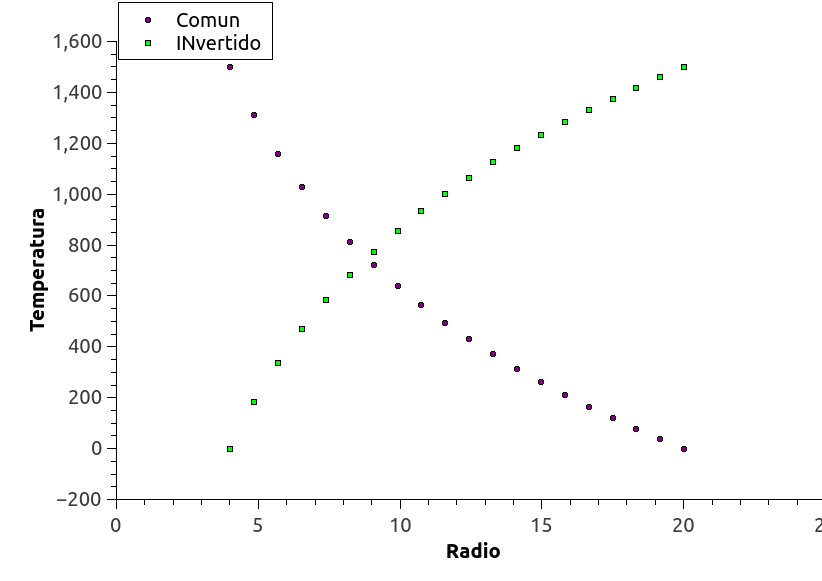
\includegraphics[scale=0.4]{imagenes/temperaturasInvertidoAmbos.png}
  \end{center}
  \vspace{-20pt}
  \caption{Temperaturas del horno con valores invertidos vs valores normales}
  \vspace{-10pt}
  \label{fig:aproximacion}
\end{wrapfigure}

Por último, el experimento 2, a pesar de ser un caso patológico, no presentó problemas a excepción de que se tuvo que adaptar la función para encontrar la isoterma, dado que no teníamos en cuenta este tipo de casos en un principio. Graficamos las temperaturas de acuerdo al radio para cada punto obtenido, y lo comparamos contra su instancia inversa, es decir, aquella que las temperaturas internas valen 1500 y las externas 0, manteninedo los demás parámetros igual. \\
Lo que sí resultó llamativo, fue hallar que los gráficos son simétricos a partir de la constante 750. Nos encontramos que, si sumamos para cada radio las temperturas de cada instancia, el resultado es siempre 1500. 

